\chapter{Introduction}\label{ch:introduction}

\section{Miscible Interiors of Sub-Neptunes}

Planets between Earth and Neptune in size are common. Among close-in Kepler planets, a gap in the
radius distribution at 1.5--2.0\,$R_\oplus$ separates smaller super-Earths from larger
sub-Neptunes \cite{fulton2017}. The larger planets are thought to be rocky interiors with
envelopes of low-density gas \cite{fulton2017}. In the evolution models discussed here, that gas
is hydrogen, and a fiducial planet of six Earth masses holds 3\% of its mass as hydrogen
\cite{rogers2025}.

Gilmore \& Stixrude \cite{gilmore2026} showed with density-functional-theory molecular dynamics
(DFT-MD) that hydrogen and liquid MgSiO$_3$ are completely miscible above a critical temperature
$T_C$. In their fit, $T_C$ falls from about 3,500\,K at 2\,GPa to 2,600\,K at 10\,GPa. They
found such conditions at the core--envelope boundary over a wide range of plausible pressures
and temperatures. Young et al.\ \cite{young2025} argued that full miscibility is the common state
of sub-Neptune interiors. The interior and the envelope then form one fluid, not a melt in
contact with a gas.

Evolution models now include this miscibility. In the models of Rogers et al.\ \cite{rogers2025}
and Rogers \& Schlichting \cite{rogers2026}, the binodal moves into the interior as the planet
cools. Hydrogen leaves the melt for the envelope as this boundary of the miscibility gap passes.
Young \& Werlen \cite{young2026} and Tang et al.\ \cite{tang2026} also couple dissolved hydrogen to
the evolution of the planet. Tang et al.\ treat its release as effectively instantaneous. These
models track where the hydrogen goes. Their energy equations do not include the heat that its
separation releases (Section~\ref{sec:interior}). Tejada Arevalo et al.\ \cite{tejada2026} study
the other side of the gap: silicate that rains out of the envelope, above a mantle that exchanges
no hydrogen with it.

\section{Heat of Exsolution}

Mixing hydrogen into silicate melt absorbs heat. The excess enthalpy of the source simulations
is positive at every simulated composition \cite{gilmore2026data}, so separation releases heat.
The process resembles crystallization, which releases latent heat. Sub-Neptune evolution
models count the latent heat of a solidifying mantle \cite{tejada2026,tang2026}. A closer
precedent is helium rain in Jupiter and Saturn, where helium demixes from metallic hydrogen.
Evolution models of these planets count the energy released as the helium sinks, mainly as
gravitational energy \cite{stevenson1977b,fortney2003,mankovich2020}. The latent heat of helium
demixing is estimated at about 200\,MJ per kg of helium. Because the droplets redissolve
deeper, it moves heat within the planet but adds none \cite{markham2024}. A miscible
sub-Neptune interior loses its hydrogen to the envelope for good, so the heat is a net source,
and its evolution models have no term for it. How large this heat is, and how it changes the
cooling of the interior, are the main questions of this work.

\section{Metastability and Delayed Exsolution}\label{sec:spinodal_intro}

Equilibrium models let hydrogen exsolve as soon as the composition enters the miscibility gap,
at the binodal \cite{rogers2025,rogers2026}. A homogeneous mixture just inside the binodal is
\emph{metastable}, however. Forming the new phase requires nucleation, which must overcome a
free-energy barrier \cite{debenedetti1996,kashchiev2000}. Only at the \textbf{spinodal} does the
mixture become unstable to small fluctuations and decompose spontaneously
\cite{cahn1958,cahn1961}. There, the curvature of the Gibbs energy with respect to composition
vanishes. Between the two lies a metastable window (Figure~\ref{fig:concept}).

\begin{figure*}[t]
\centering
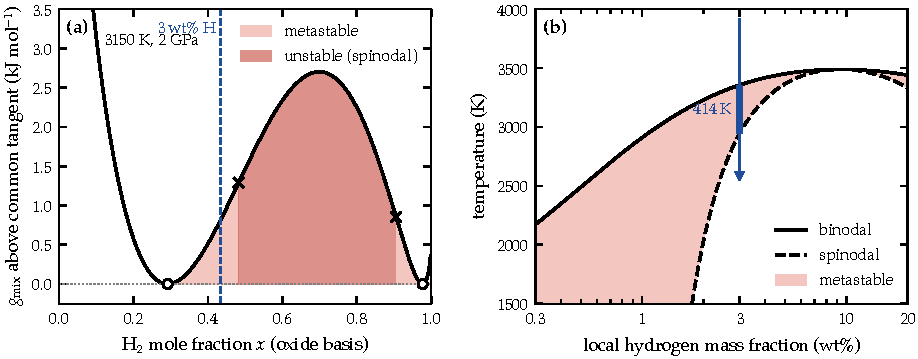
\includegraphics[width=\textwidth]{fig1_1_concept}
\thesiscaption{Binodal, spinodal and the metastable window of a cooling H$_2$--MgSiO$_3$
parcel.}{(a) Homogeneous Gibbs energy of mixing at 2\,GPa and 3150\,K above its common
tangent, for the published mixing model \cite{gilmore2026}. Circles mark the coexisting
compositions (binodal), crosses the inflection points (spinodal). A parcel with 3\,wt\%
local hydrogen (dashed line) is metastable here. (b) Binodal and spinodal temperatures at
2\,GPa as a function of local hydrogen mass fraction. A 3\,wt\% parcel cooling at fixed
pressure (arrow) enters the miscibility gap at the binodal but becomes unstable only at the
spinodal.}
\label{fig:concept}
\end{figure*}

Young et al.\ \cite{young2025} already plotted the binodal, the spinodal and this window for
H$_2$--MgSiO$_3$ (their Fig.~2), using the 2025 preprint fit \cite{stixrude2025}. They did not ask how
long the window delays separation, or whether nucleation lets a cooling parcel reach the
spinodal. In silicate magmas, delayed degassing through suppressed nucleation is well documented
\cite{mangan2000}, and nucleation on crystals and other interfaces may dominate \cite{shea2017}.
Nishiwaki \cite{nishiwaki2025} derived a spinodal for hydrous magma from solubility data through
an assumed solution model.

Such an inference has a known weakness. The spinodal is a property of the homogeneous free energy
inside the gap, and simulations of coexisting phases do not sample that state. A spinodal
derived from a fitted mixing model therefore inherits the assumed functional form. We test how
far the existing data constrain it.

\section{Contributions and Scope}

We study binary H$_2$--MgSiO$_3$ mixtures with the 2026 mixing model \cite{gilmore2026} and its
source simulations \cite{gilmore2026data}. We cover local hydrogen mass fractions of 0.1--20\%,
pressures of 2--10\,GPa and temperatures of 2,000--4,000\,K. The local mass fractions describe
the melt at the top of the interior, not the hydrogen budget of the whole planet. This work makes
four contributions.
\begin{enumerate}
\item \textbf{Open-source tools.} We add energy, nucleation and cooling-path functions to the
open-source code \Atm{} \cite{bower2025}, with a composition-consistent basis for the 2026
model. A separate scalar code reproduces the \Atm{} binodals and spinodals to within
\indepMaxDiff{}\,K. The full \Atm{} equilibrium solver reproduces the mixing enthalpy along
one published-fit parcel path (3\,wt\% at 2\,GPa, separating at the spinodal) to a relative
difference of $\replayDiff{}$ over \replayRows{} solves (Section~\ref{sec:verification} and
Appendix~\ref{app:repro}).
\item \textbf{The heat of exsolution.} We compute the heat released per kilogram of exsolved
hydrogen from the same free energy that sets the binodal. We test it against the simulated excess
enthalpies and follow its effect on a convecting interior (Sections~\ref{sec:heat}
and~\ref{sec:interior}).
\item \textbf{Near-equilibrium kinetics.} We compute the homogeneous nucleation barrier in
square-gradient theory. It ends metastability \dlyFigOneCPubLo{}--\dlyFigOneCPubHi{}\,K below
the binodal for the published fit (Section~\ref{sec:kinetics}).
\item \textbf{What the source data constrain.} We audit the published fit against its source
simulations and refit four model classes. The data constrain the heat, but they do not fix the
spinodal (Sections~\ref{sec:audit}--\ref{sec:identifiability}).
\end{enumerate}

We do not run a planetary evolution model. The convecting interior is well mixed, and its
composition follows the hydrogen-poor binodal at its top (Section~\ref{sec:interior}). The
planet-wide estimate post-processes a published energy budget \cite{rogers2025}. The mixture
contains no helium or iron. Like the source fit, all model classes take the excess enthalpy,
entropy and volume as independent of temperature.
